\section{Ejercicio 3: Crear un panel de Power BI - Tarea 2: Crear un Panel de Power BI} 

1. In Power BI, in the top-left corner, click Show the navigation pane.\\
2. Under Reports, click AdventureWorksLT Sales.\\
3. At the bottom of the page, click Page 1, click the Target Sales visual, and then click Pin visual.\\

	\begin{center}
	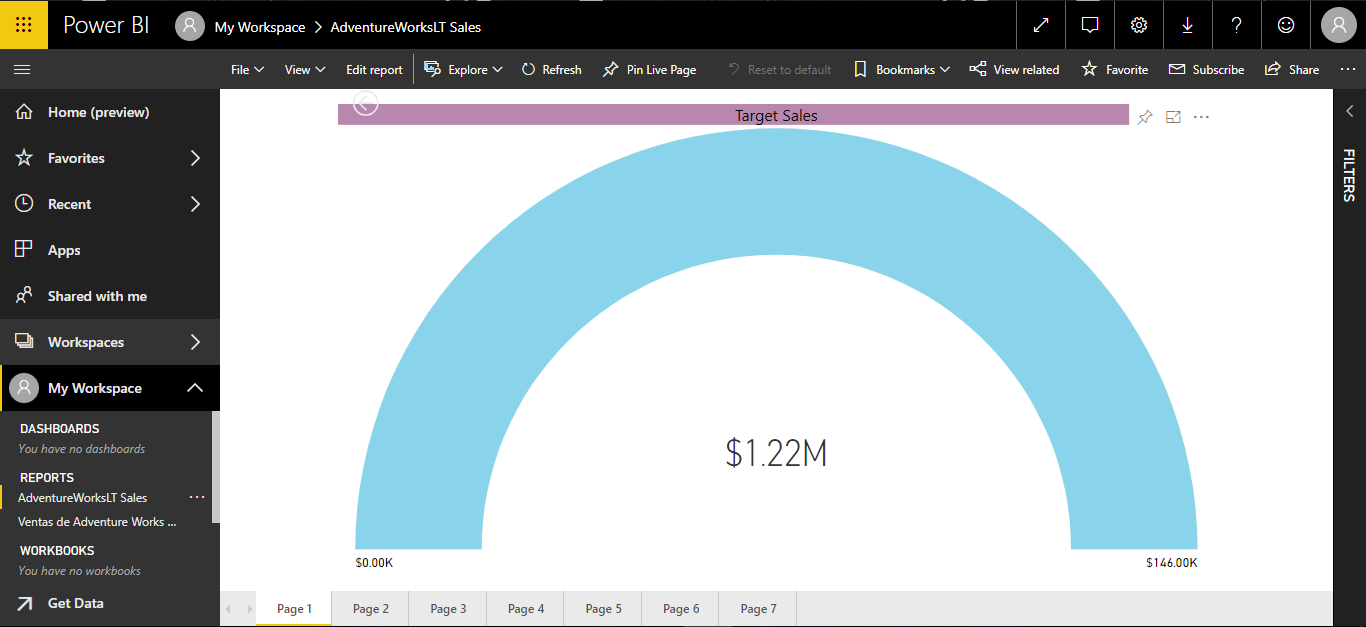
\includegraphics[width=17cm]{./Imagenes/Ejercicio3/Tarea2/1}
	\end{center}	

4. In the Pin to dashboard dialog box, click New dashboard, type AdventureWorksLT Sales, and
then click Pin.\\

	\begin{center}
	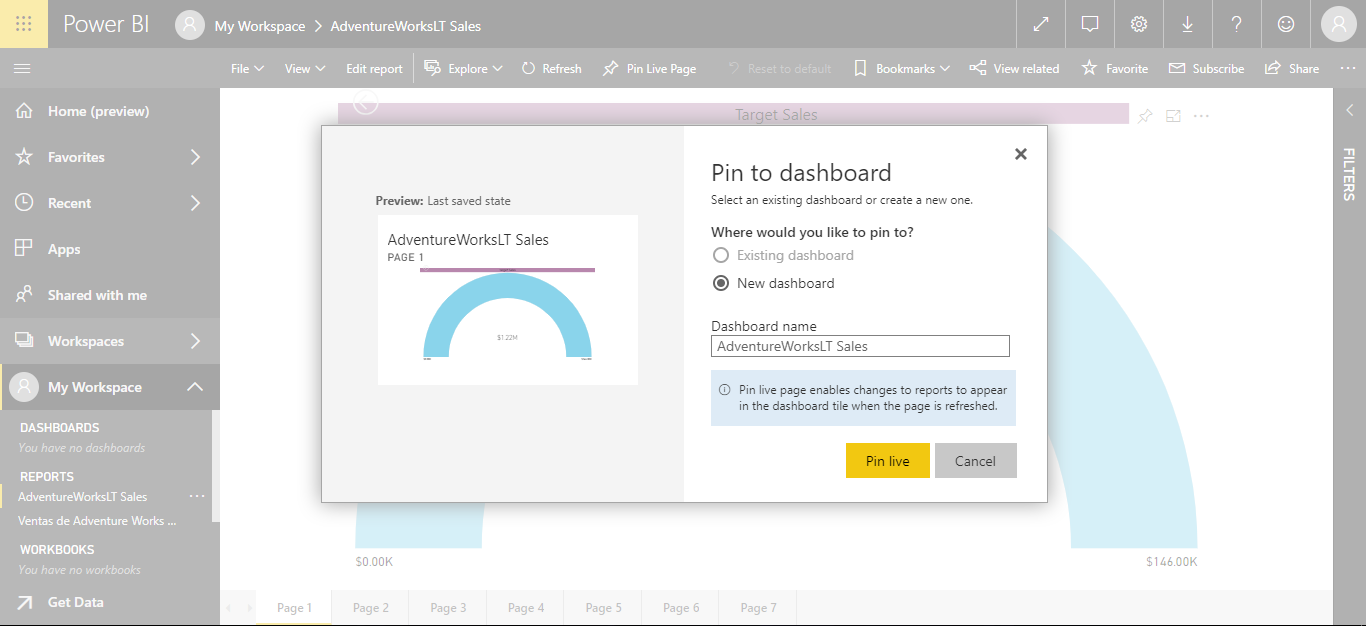
\includegraphics[width=17cm]{./Imagenes/Ejercicio3/Tarea2/2}
	\end{center}	

5. On the Top Selling Customers visual, click Pin visual.\\

	\begin{center}
	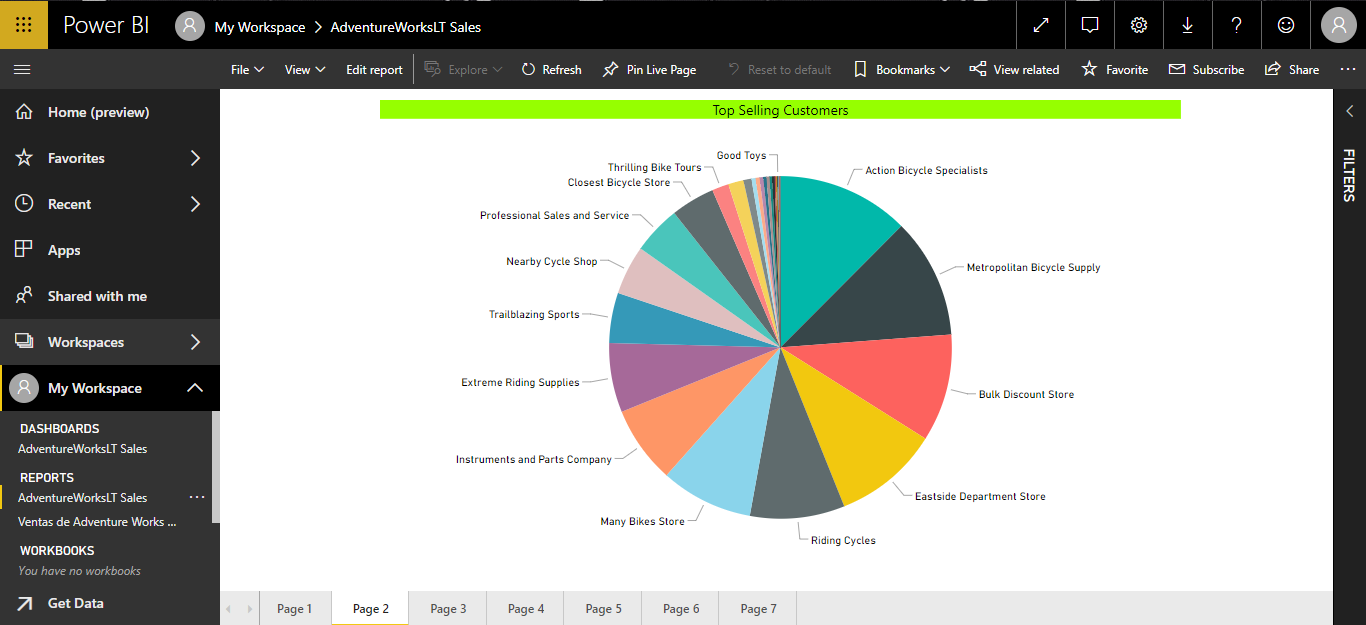
\includegraphics[width=17cm]{./Imagenes/Ejercicio3/Tarea2/3}
	\end{center}	

6. In the Pin to dashboard dialog box, click Existing dashboard, in the list, click AdventureWorksLT
Sales, and then click Pin.\\

	\begin{center}
	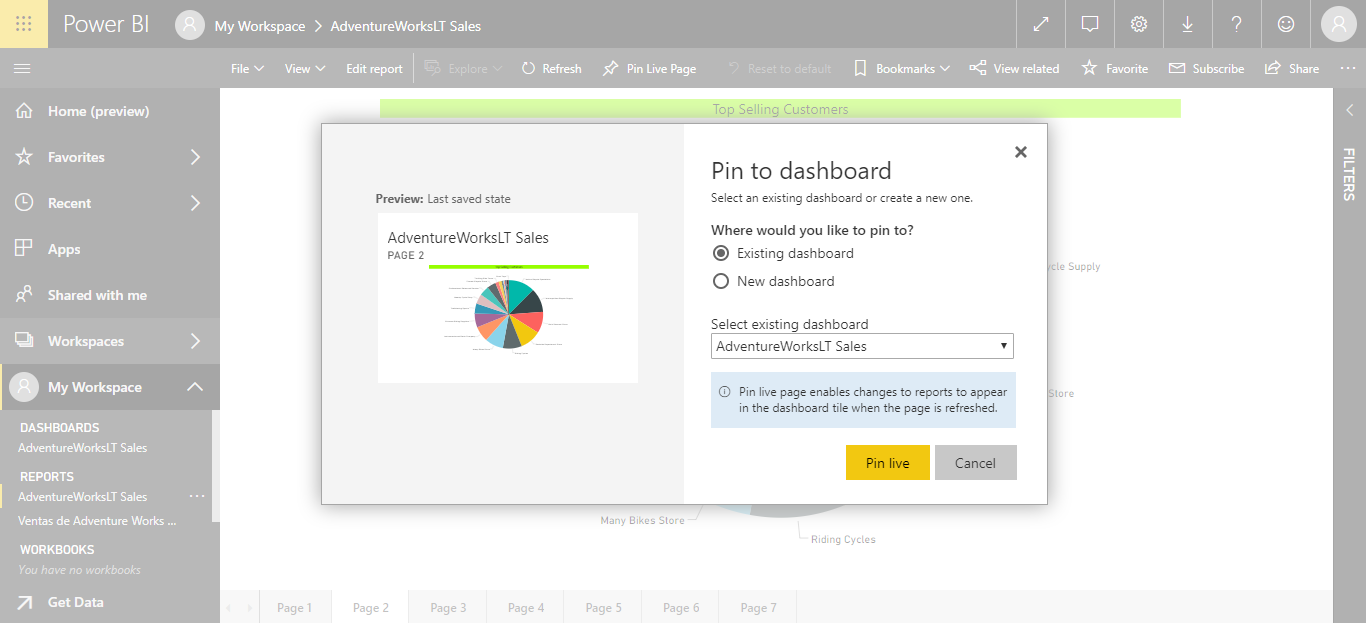
\includegraphics[width=17cm]{./Imagenes/Ejercicio3/Tarea2/4}
	\end{center}	

7. On the Orders by Main Category visual, click Pin visual.\\

	\begin{center}
	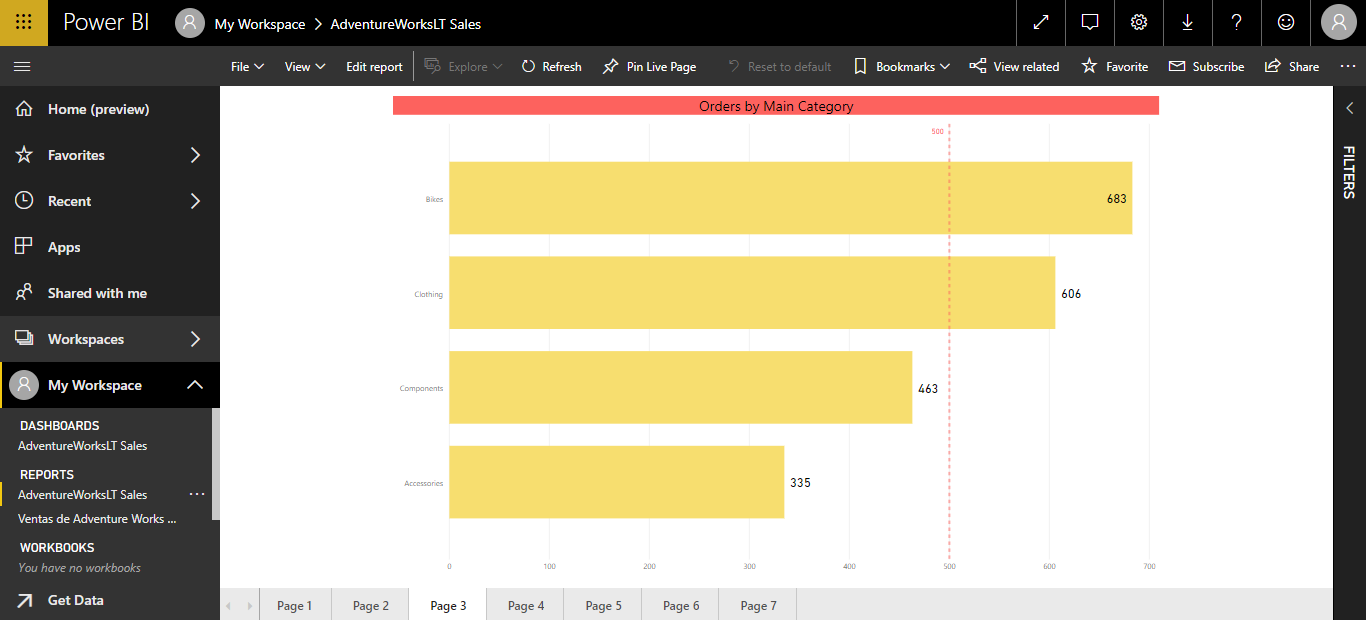
\includegraphics[width=17cm]{./Imagenes/Ejercicio3/Tarea2/5}
	\end{center}	

8. In the Pin to dashboard dialog box, click Existing dashboard, in the list, click AdventureWorksLT
Sales, and then click Pin.\\

	\begin{center}
	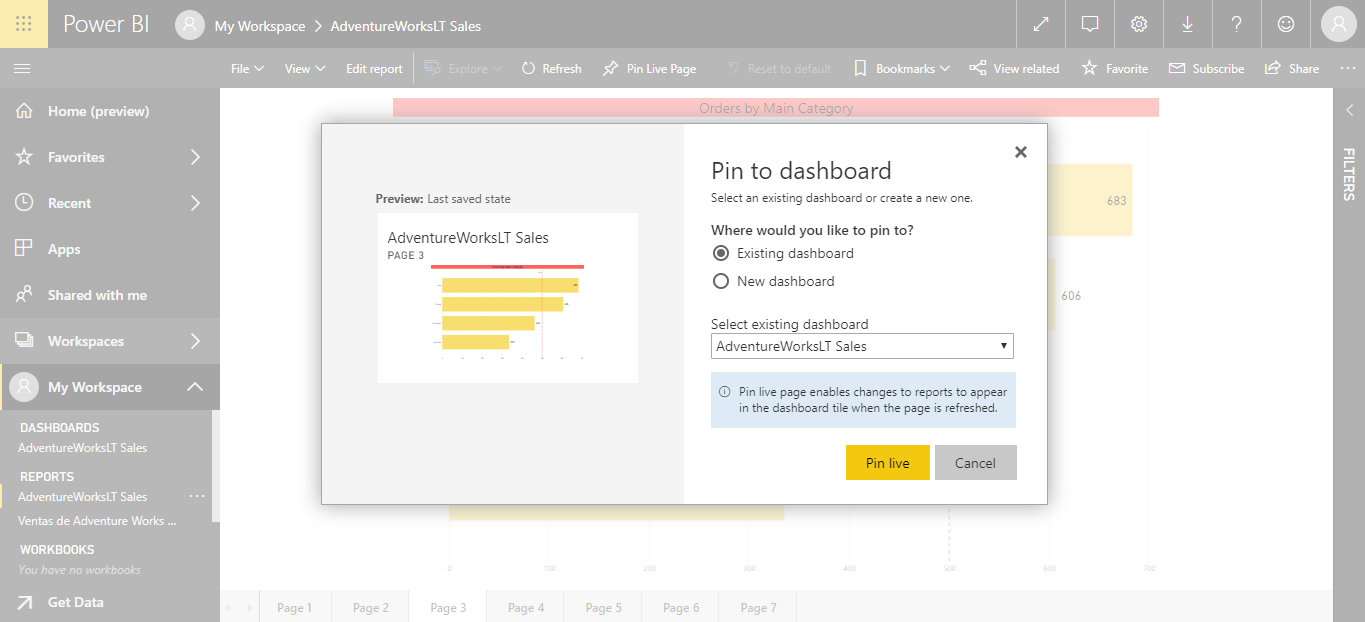
\includegraphics[width=17cm]{./Imagenes/Ejercicio3/Tarea2/6}
	\end{center}	

9. On the Top 10 Selling Bikes visual, click Pin visual.\\

	\begin{center}
	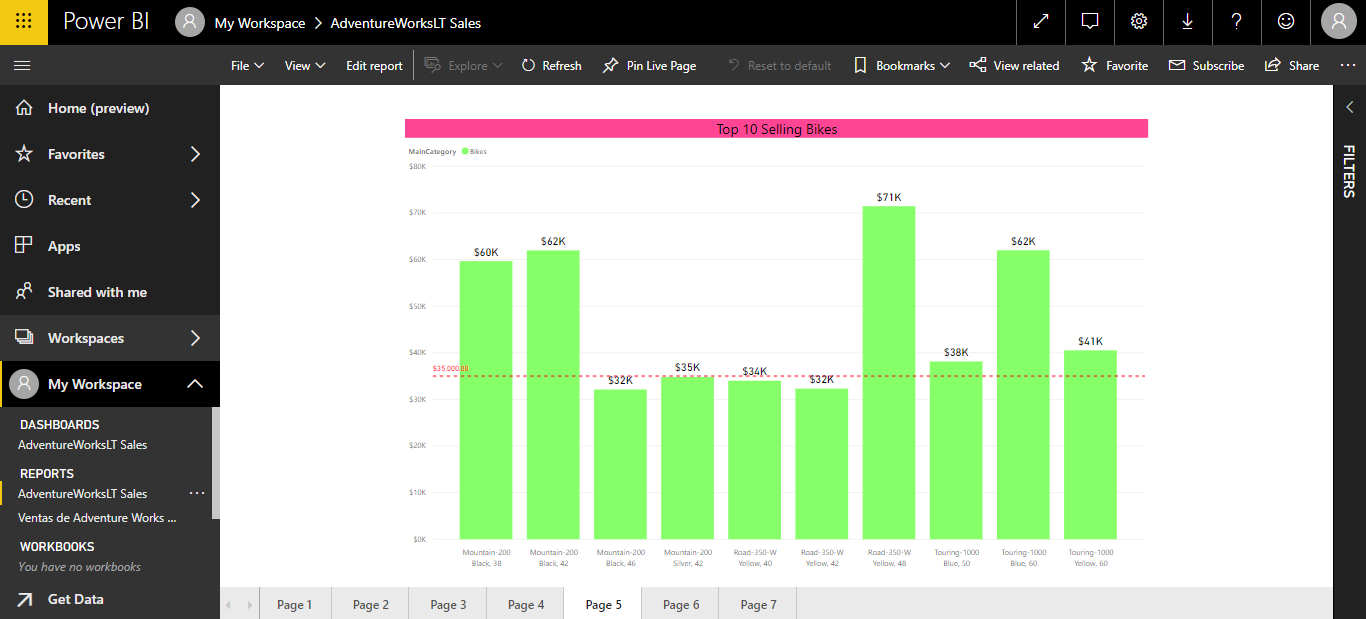
\includegraphics[width=17cm]{./Imagenes/Ejercicio3/Tarea2/7}
	\end{center}	

10. In the Pin to dashboard dialog box, click Existing dashboard, in the list, click AdventureWorksLT
Sales, and then click Pin.\\

	\begin{center}
	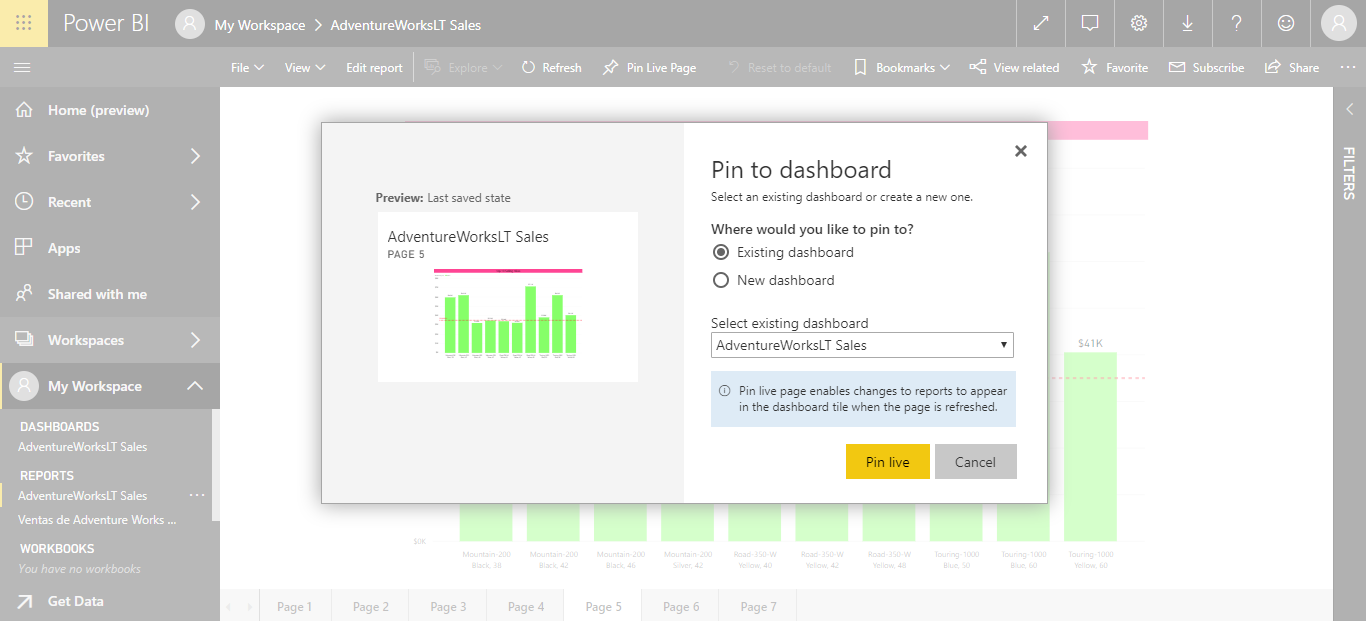
\includegraphics[width=17cm]{./Imagenes/Ejercicio3/Tarea2/8}
	\end{center}	

11. On the Sales by Main Category visual, click Pin visual.\\

	\begin{center}
	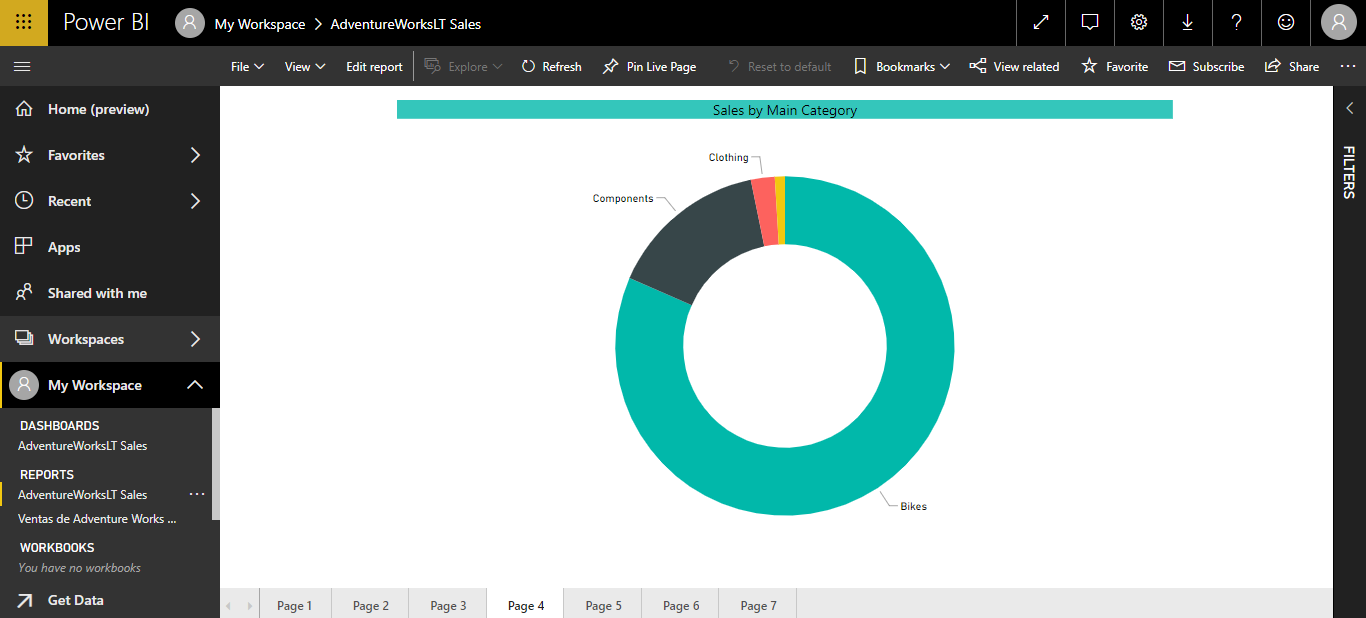
\includegraphics[width=17cm]{./Imagenes/Ejercicio3/Tarea2/9}
	\end{center}	

12. In the Pin to dashboard dialog box, click Existing dashboard, in the list, click AdventureWorksLT
Sales, and then click Pin.\\

	\begin{center}
	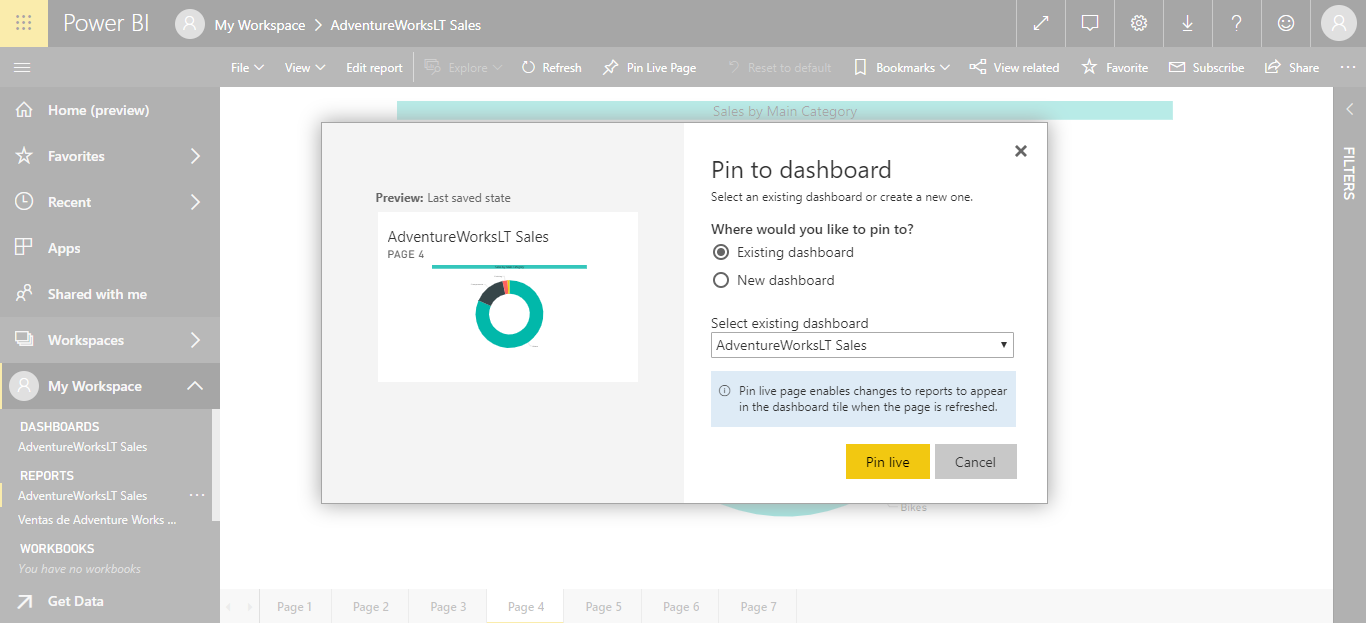
\includegraphics[width=17cm]{./Imagenes/Ejercicio3/Tarea2/10}
	\end{center}	

13. The dashboard is listed in the My Workspace pane, under Dashboards. Notice the yellow star icon
to denote that this is a new dashboard.\\
14. Click the AdventureWorksLT Sales dashboard to open it.\\
15. Notice that the tiles are all the same size.\\
16. On the Target Sales tile, click Open menu (…), and then click Tile details.\\
17. In the Subtitle box, type Sales target for 2016, and then click Apply.\\

	\begin{center}
	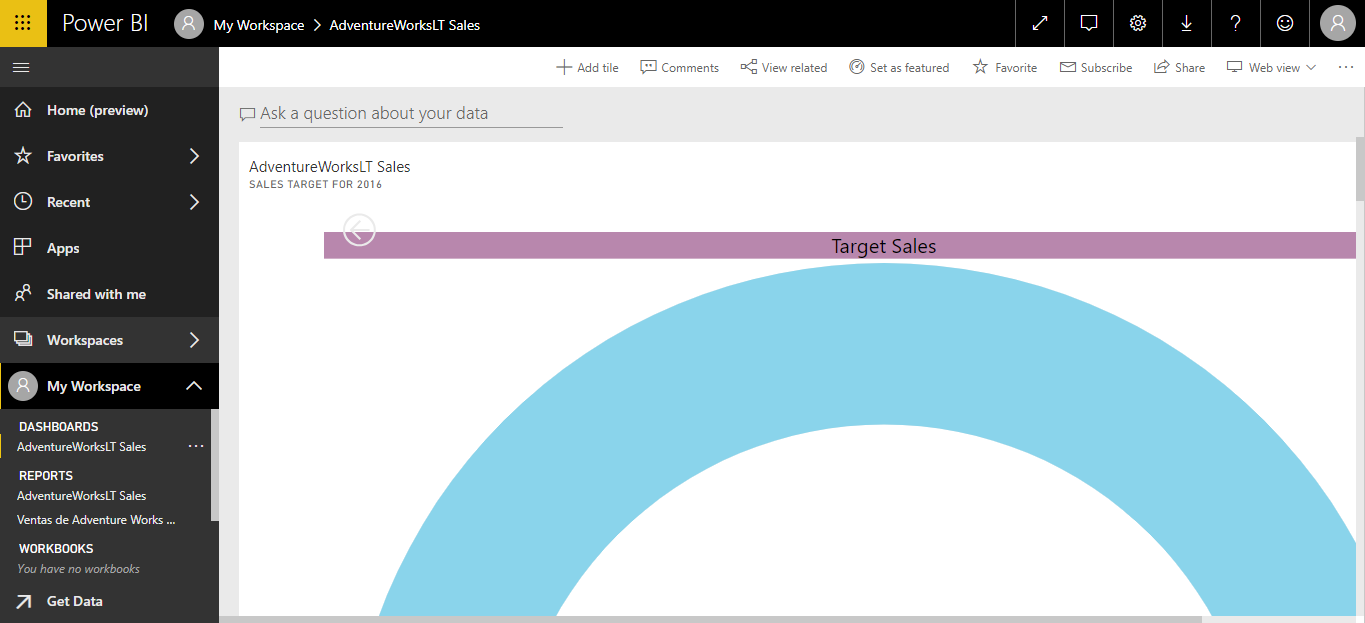
\includegraphics[width=17cm]{./Imagenes/Ejercicio3/Tarea2/11}
	\end{center}	

18. On the Top Selling Customers tile, click Open menu (…), and then click Tile details.\\
19. In the Subtitle box, type Customers selling the most products, and then click Apply.\\

	\begin{center}
	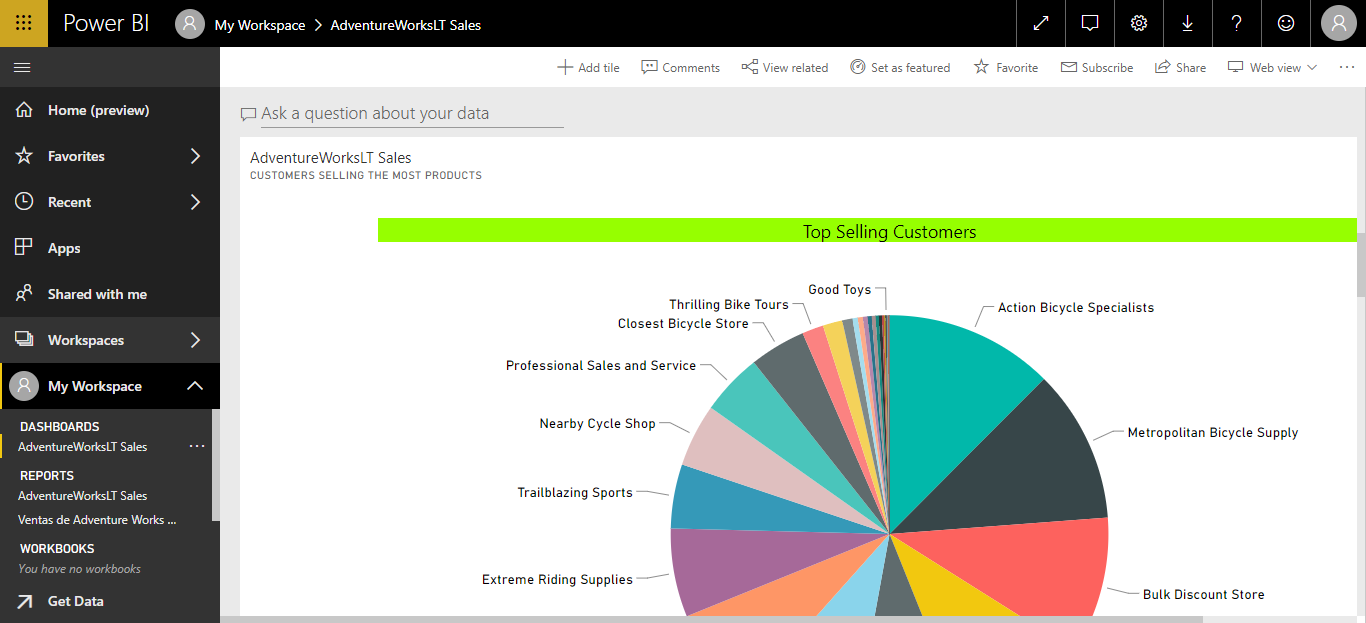
\includegraphics[width=17cm]{./Imagenes/Ejercicio3/Tarea2/12}
	\end{center}	

20. On the Top 10 Selling Bikes tile, click Focus mode. The tile opens into its own space.\\
21. Expand the Filters pane, expand LineTotal, change the value of 32000 to 40000, and then click Apply filter.\\
22. Next to the report title, TOP 10 SELLING BIKES, click the Back to AdventureWorksLT Sales button.\\
23. Click Enter Full Screen Mode. Notice that the dashboard displays without any of the browser
interface. This is ideal for presentations.\\

	\begin{center}
	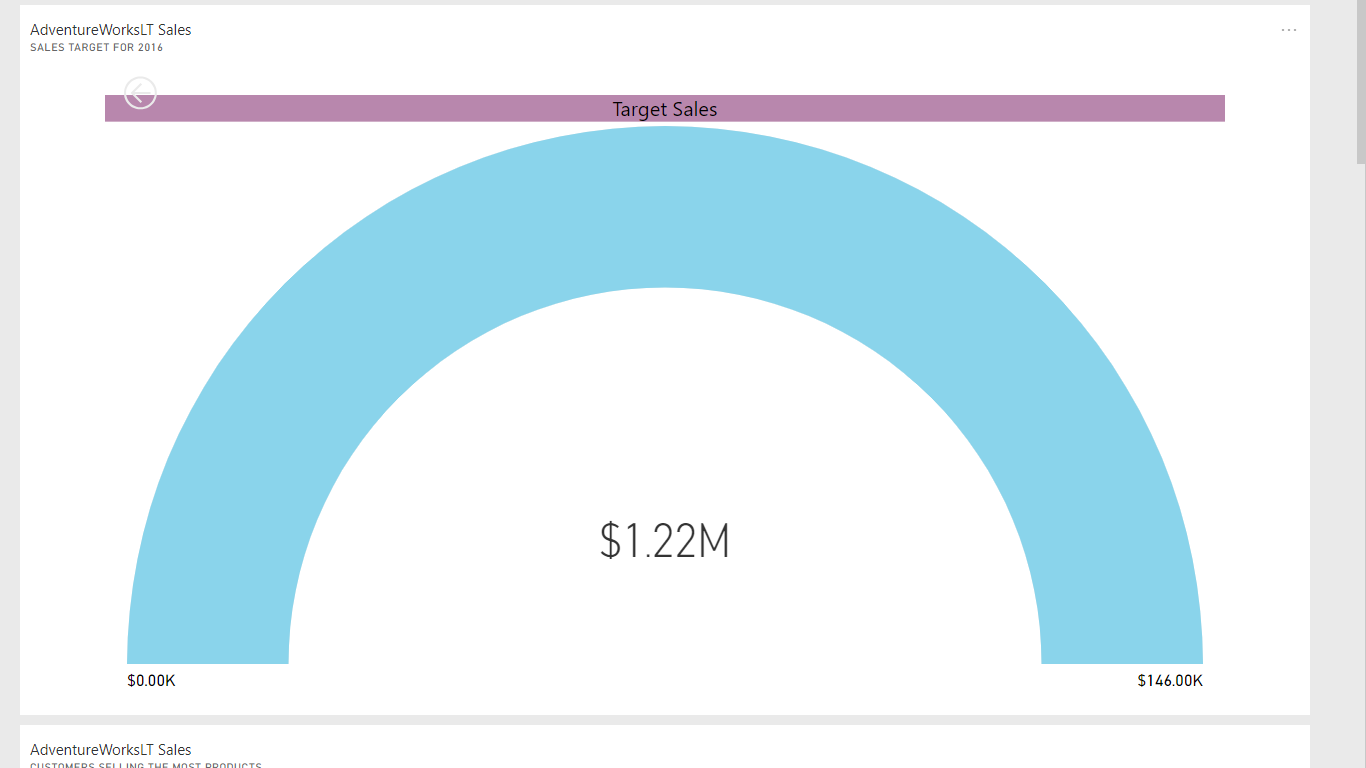
\includegraphics[width=17cm]{./Imagenes/Ejercicio3/Tarea2/13}
	\end{center}	

24. Press Esc to exit full-screen mode, and return to the dashboard.\\
25. Close Internet Explorer.\\
26. In the Publishing to Power BI window, click Got it.\\
27. Close Power BI Desktop, and then close Excel and SQL Server Management Studio without saving any
changes.

